%%%%%%%%%%%%%%%%%%%% INTRO %%%%%%%%%%%%%%%%%%%%%%%%%%
\section{Overview}\label{eval:introduction}

In the last few years, significant improvements in both hardware and software have led to a proliferation of AR applications for mobile devices and AR headsets, and extensive research has been conducted on the integration of AR in education \citep{7943075, akccayir2017advantages, chen2017new, ibanez2018augmented, pellas2019augmenting, 10.3897/jucs.76535}. However, despite these advancements and research efforts, the use of AR in primary and secondary schools is still not common \citep{doi/10.2759/121671}.
The main reasons behind this were identified in Chapters \ref{chap:sota} and \ref{chap:arch}, namely the limited collaboration capabilities of existing apps, the inability to create new content and the difficulty of adapting to existing school curricula.
In Chapter \ref{chap:arch}, \arch{} was presented as an interoperable architecture. It enables the creation of multi-user AR applications and simplifies the development process. \arch{} also allows the stakeholders to add new content to existing applications, track user progress and integrate application data into the \gls{lms} used by the teachers.

The analysis of the answers provided by the teachers allowed the identification of 6 \glspl{do}, as described in Section \ref{arch:architecture}. A conceptual evaluation of the \arch{} architecture was performed through the creation of 3 \glspl{poc} (presented in Section \ref{arch:implementation}). The aim of this initial evaluation was to demonstrate that \arch{} fulfils the aforementioned \glspl{do}.

% \begin{itemize}
%  \item \textbf{Interoperability (DO1)}: The architecture enables the creation of applications that can run on multiple devices \textendash{} tablets, smartphones, \glspl{hmd} or laptops \textendash{} and provide APIs for development on multiple platforms.
%  \item \textbf{Multi-user capabilities (DO2)}: As collaboration is a key requirement, the architecture provides tools to support multi-user functionalities, both for remote and in-class collaboration.
%  \item \textbf{Data analytics (DO3)}: The architecture enables long-term data storage as well as tools for automatic data analysis and visualization, by providing an API to access standard dataviz and machine learning libraries.
%  \item \textbf{Easy to develop (DO4)}: The applications relying on the architecture can be developed quickly and easily.
%  \end{itemize}
 
% In the previous Chapter, three \glspl{poc} were described. Their aim is to perform a conceptual evaluation of the architecture and to demonstrate that it fulfills the aforementioned \glspl{do}.

This new Chapter builds upon such previous work and introduces \appname{}, a multiplatform collaborative AR geography game.
The primary goal of the application is to demonstrate the potential of the \arch{} architecture for creating interoperable applications that can be integrated into school curricula\footnote{The application is open source and the code can be accessed at \url{https://github.com/tv-vicomtech/ARoundtheworld}}.
Additionally, the game aims to enhance student engagement through the collaborative functionalities provided by \arch{}.
%how collaborative \gls{ar} applications built using the cleAR architecture can increase students' engagement and be easily included in school curricula, thanks to its integration and customisation capabilities.
The application has been developed incorporating feedback from the teachers of a Basque primary and secondary school association\footnote{\url{https://ikastola.eus/}} and it has been evaluated after being tested with \numstudents/ students in three different educational institutions.
Once the test was complete, teachers were interviewed while students were asked to fill in a short questionnaire about the \appname{} \gls{ui} and the \gls{ux} it offered. The questionnaire also asked about the app effectiveness as a tool for raising the engagement of the students and enabling collaboration between them.
To perform a quantitative evaluation about \appname{} collaboration capabilities, the app collected data \textendash{} in the form of xAPI statements \citep{xAPIspec} \textendash{} about its usage, the number of interactions between students and their performance.

The choice of Geography as the application domain is motivated by the fact that geographical exploration is an integral part of child development \citep{catling1993whole}, and the use of maps helps students improve spatial thinking skills \citep{collins2018impact}.
The application is structured as a quiz where students take turns to answer Geography questions.
If a student is struggling to answer a question, other students can interact in the augmented space and provide hints to the active user.
\appname{} works both as a mobile and a web application, is easily extensible and provides several logging and tracking mechanisms, which can be easily integrated into the \gls{lms} of the school to enable automatic tracking of the progress of the students.

The main contributions of this Chapter can be summarised as:
\begin{itemize}
    \item A complete description of the application and the feasibility of implementing the different components of the \arch{} architecture to fulfil all the design objectives.
    \item A qualitative evaluation of the technology integrated in the application, based on the questionnaires filled in by the \numstudents/ students and the interviews with their teachers.
    \item An analysis of the data collected by the application during the user study, with a focus on the effects of collaboration capabilities on the quiz results and the engagement of the students.
\end{itemize}

The number of users who participated in the study is not representative of the whole student population. The aim, in this case, is not to demonstrate the positive effects of AR in schools, but rather to validate the architecture presented in a real educational setting, and not only through the development of PoCs.

The rest of the Chapter is structured as follows: Section \ref{eval:related} covers the relevant state of the art.
Section \ref{eval:appdesc} describes the implementation details of \appname{}, while Section \ref{eval:evaluation} outlines our methodological framework and the evaluation process.
In Section \ref{eval:results}, the results obtained from the student questionnaires and teacher interviews are described, together with the quantitative analysis of the data collected through the application.
Finally, Section \ref{eval:conclusion} presents some final remarks. 

%%%%%%%%%%%%%%%%%%%% RELATED %%%%%%%%%%%%%%%%%%%%%%%%
\section{Related Work}\label{eval:related}

A recent review of AR applications used in education \citep{eleniiattro} mentions that collaborative learning in AR represents a critical research direction, but so far very few studies provide collaborative functionalities in an AR environment \citep{9645428, choi2017arclassnote}.
The work from \cite{cai2017applications} presents an application that makes use of a Kinect camera to extract 3D information from the scene and display virtual magnetic induction lines.
In \citep{takahashi2018empathic}, the authors designed a large scale AR and projection system, modifying the gymnasium of the school, to create a learning game for children with \gls{asd}, which was designed to keep their attention focused on the content provided.
\cite{laviole2018nectar} presented a markerless application for learning how an artificial neural network works, where the students can manually tweak the values of the network parameters and see how it affects the ability of the network to classify images.

As it heavily relies on visual representation of data, several technologies have been exploited to make the teaching of Geography more effective and engaging.
In the context of AR, \cite{palaigeorgiou2018touching} used a projector to create tangible 3D maps with which up to three students could interact at the same time.
\cite{xefteris2019mixing} extended the concept of tangible maps by including the usage of programmable robots to guide the students through a virtual journey. A collaborative AR app for teaching geography and geology is the one presented in \citep{wellmann2022open}. The app relies on a AR sandbox\footnote{\url{https://ar-sandbox.eu/}} to display the content and it allows teacher to modify its behaviour by writing code in the form of Jupyter notebooks.

As far as evaluating the effectiveness of AR applications for education, the vast majority of the studies highlight a positive (albeit limited) effect derived from using the technology.
\cite{CHANG2022104641} performed a meta-analysis of 134 studies which suggests that AR benefits all the learning outcomes evaluated, with the largest effect being on students performance.
A systematic review of 45 studies \citep{da2019perspectives} reaches the same conclusions, but highlights the many differences in the evaluation protocols, which complicate the statistical analysis of AR effectiveness across different applications.

AR applications are often implemented as serious games, in which using gamification concepts the students can more easily learn and retain concepts that would otherwise not interest them.
\cite{oh2017hybrid} described a game-based simulation where the users can study the properties of light such as reflection and refraction.
\cite{lopez2020emofindar} created a multiplayer game in which children can improve their communication skills by practicing in an AR environment, while \cite{ccelik2022use} described a gamified AR app used in a Content and Language Integrated class.

Several publications focus on the importance of effective \glspl{ui} and \glspl{ux} in enhancing student engagement.
A systematic review of the literature analysed 49 studies \citep{LAW2021100321} and identified a lack of information about usability and user experience frameworks, suggesting that there is a disconnect between Human-Computer Interaction (HCI) and \gls{tel} communities, as well as a lack of AR-specific \gls{ux} evaluation metrics.
The work of \cite{thamrongrat2019design} evaluated the learning effect for teaching 3D geometry using an AR application compared to traditional learning, as well as the user engagement of the students using the app compared to the ones in the control group.
Another study \citep{alrashidi2017evaluating} compared the effectiveness of learning software debugging concepts using an AR application versus a non-AR approach.

Applications used in schools usually generate data that are stored on the school \gls{lms}.
A standard that is recently gaining traction for collecting data about the activities of the learners is eXperience API, an open-source software specification that makes it possible to collect data about a wide range of learning experiences. This is achieved by sending each activity that needs to be recorded to a \gls{lrs} in a consistent and secure format \citep{xAPIspec}.
The activities are collected as statements stored as JSON objects.
Statements can be tuned to a specific use case by defining a vocabulary of valid statements.
\cite{9225931} described a system where xAPI is used to perform learning analytics in an AR environment, while \cite{wu2020design} used xAPI to collect data for a 3D design course.

%%%%%%%%%%%%%%%%%%%% APP DESC %%%%%%%%%%%%%%%%%%%%%%%
\section{Collaborative AR application}\label{eval:appdesc}

This Section describes how the application is implemented and how the developed application fulfils the \gls{do}s presented in Section \ref{arch:req:desobj}.
The application, called \appname{}, is a collaborative geography quiz in which students answer a set of questions prepared by the teacher.
Once started, the application sends a question to the first student (for example, \textit{Where is Kyoto?}). The student answers by placing a pin on the 3D globe of the Earth shown in the augmented space.
Other students can collaborate with the active user in two ways. They can suggest to her in which continent the answer is located and \textendash{} once the user has placed the pin but has not confirmed her choice yet \textendash{} by sending a \textit{thumbs up} or \textit{thumbs down} feedback\footnote{A video description of the application is available at this link: \url{https://anon.to/a7NPy8}}.
Once a student answers, the application sends a new question to the next user, and repeats the process until all the questions have been answered.
Figure \ref{fig:app_workflow} shows the application workflow, highlighting the interactions of teacher and students.

\begin{figure*}[htbp]
    \centering
    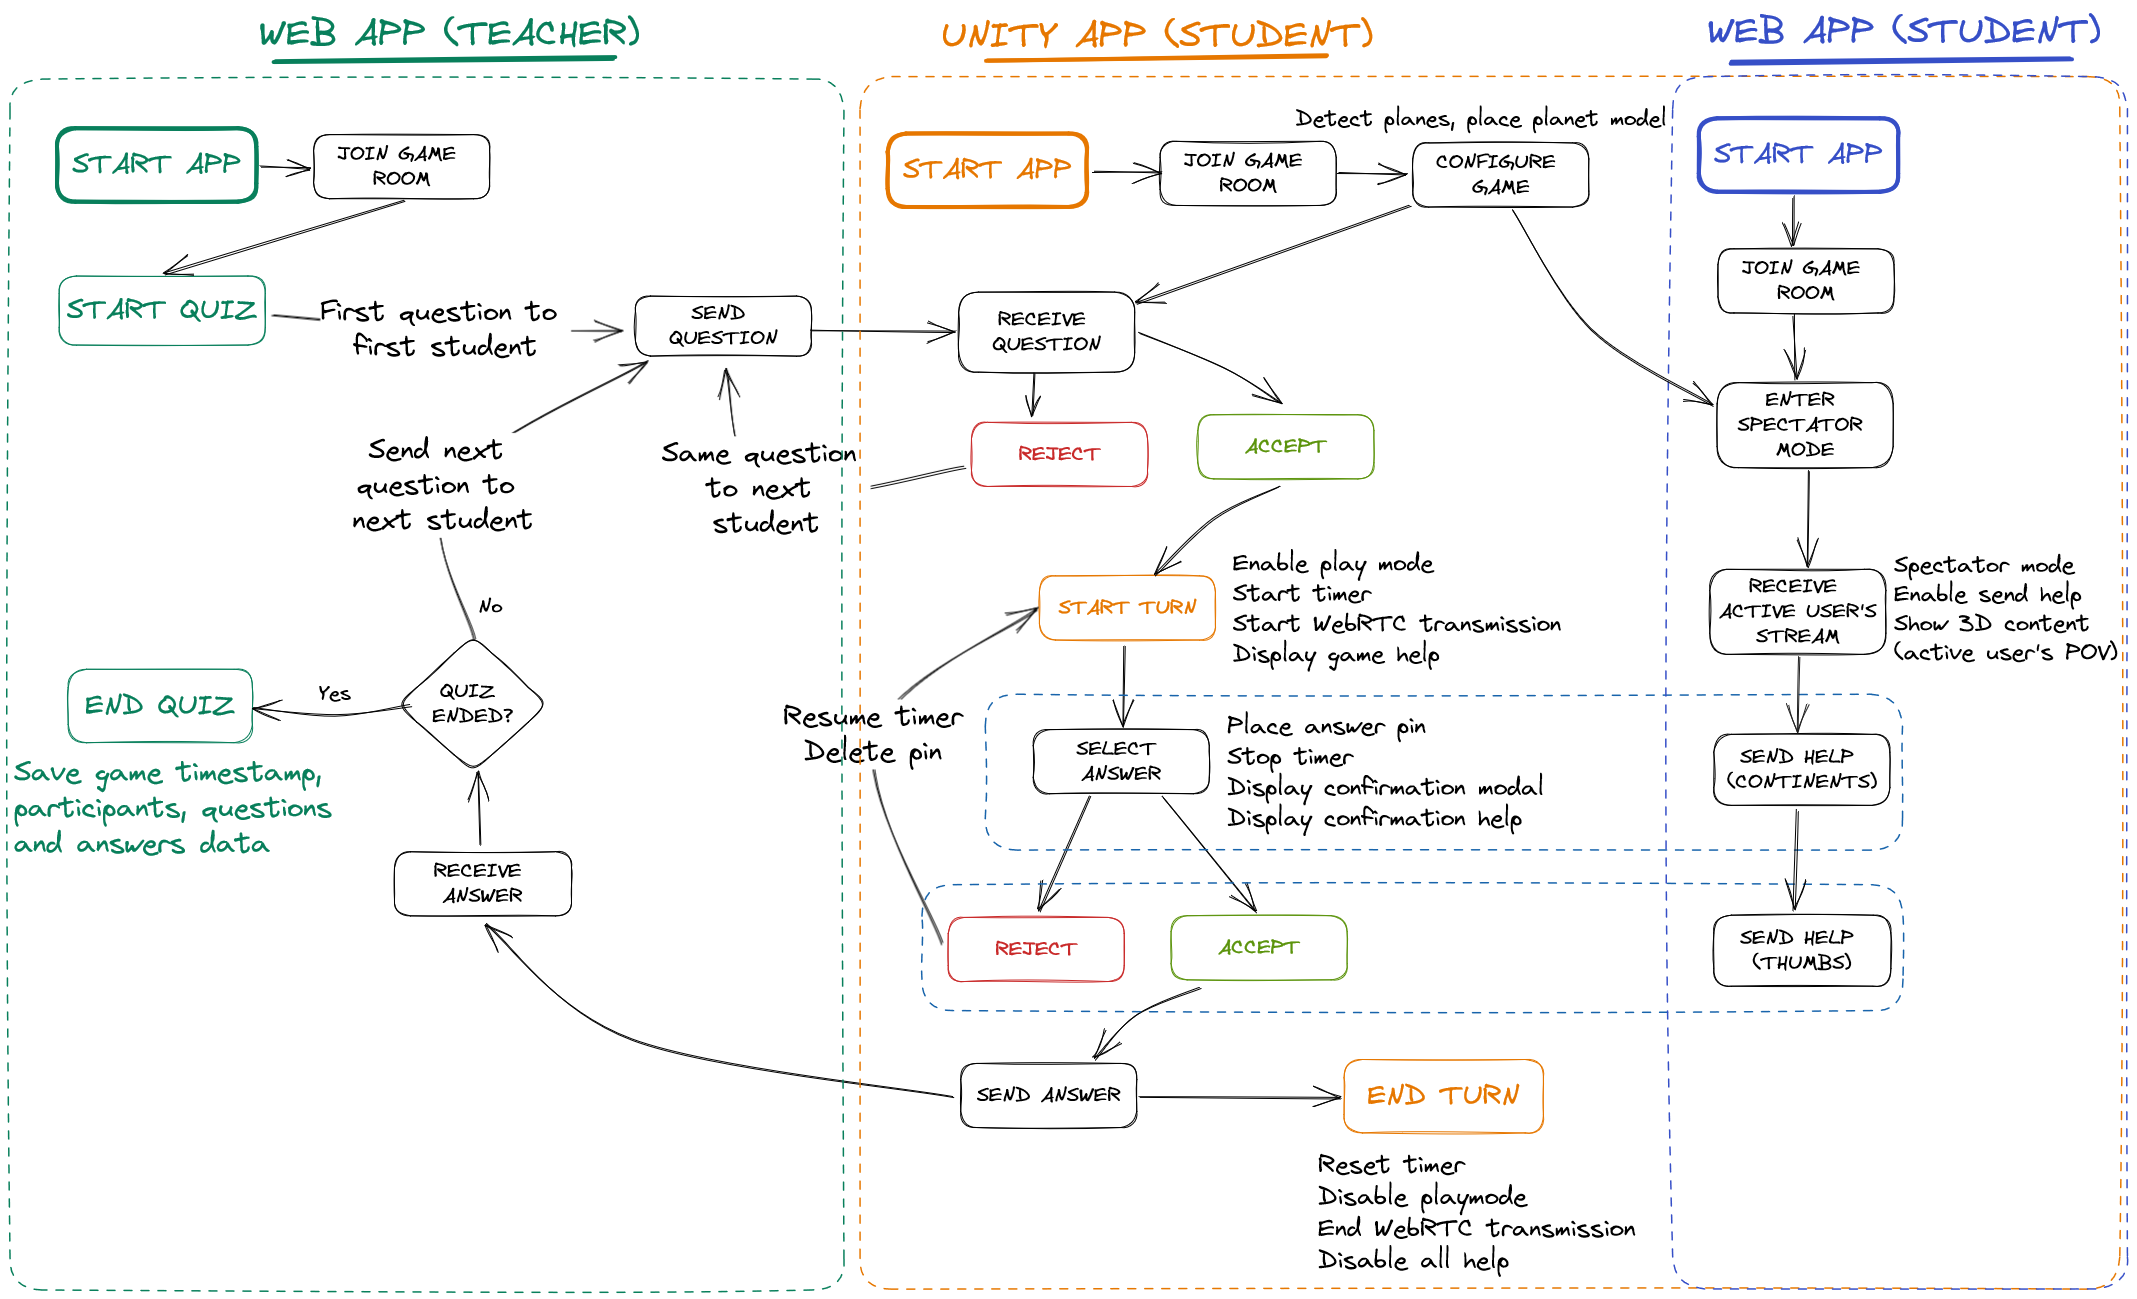
\includegraphics[width=0.95\textwidth]{workflow_diagram_3.png}
    \caption{\fontsize{10pt}{11pt}\selectfont{\itshape{Workflow of the \appname{} application.}}}
    \label{fig:app_workflow}
\end{figure*}

%Figure \ref{fig:student_interface} shows the interface of the application for a user once she receives a question

%\begin{figure}[htbp]
%    \centering
%    \includegraphics[width=0.4\textwidth]{UnityStudent_6.PNG}
%    \caption[The AR interface used by students participating to the quiz.]{The AR interface used by students participating to the quiz.}
%    \label{fig:student_interface}
%\end{figure}

The application considers three types of users (\textit{teacher}, \textit{players} and \textit{watchers}), depending on their role and their means of interacting with other users.
The first role is that of the students participating in the quiz, \textendash{} the \textit{player} \textendash{} described above.
Another role is that of the \textit{teacher}, who controls the overall status of the app through a web-based interface.
The final role \textendash{} the \textit{watcher} \textendash{} is that of the students who are not actively participating in the quiz (i.e., they are not answering any questions). They can watch what other students are doing and give them clues to find the correct answer.
This role was designed to let students without an AR capable device engage with the players by checking what they are doing and collaborate with them by suggesting the correct answer.

\begin{figure*}[t]
    \centering
    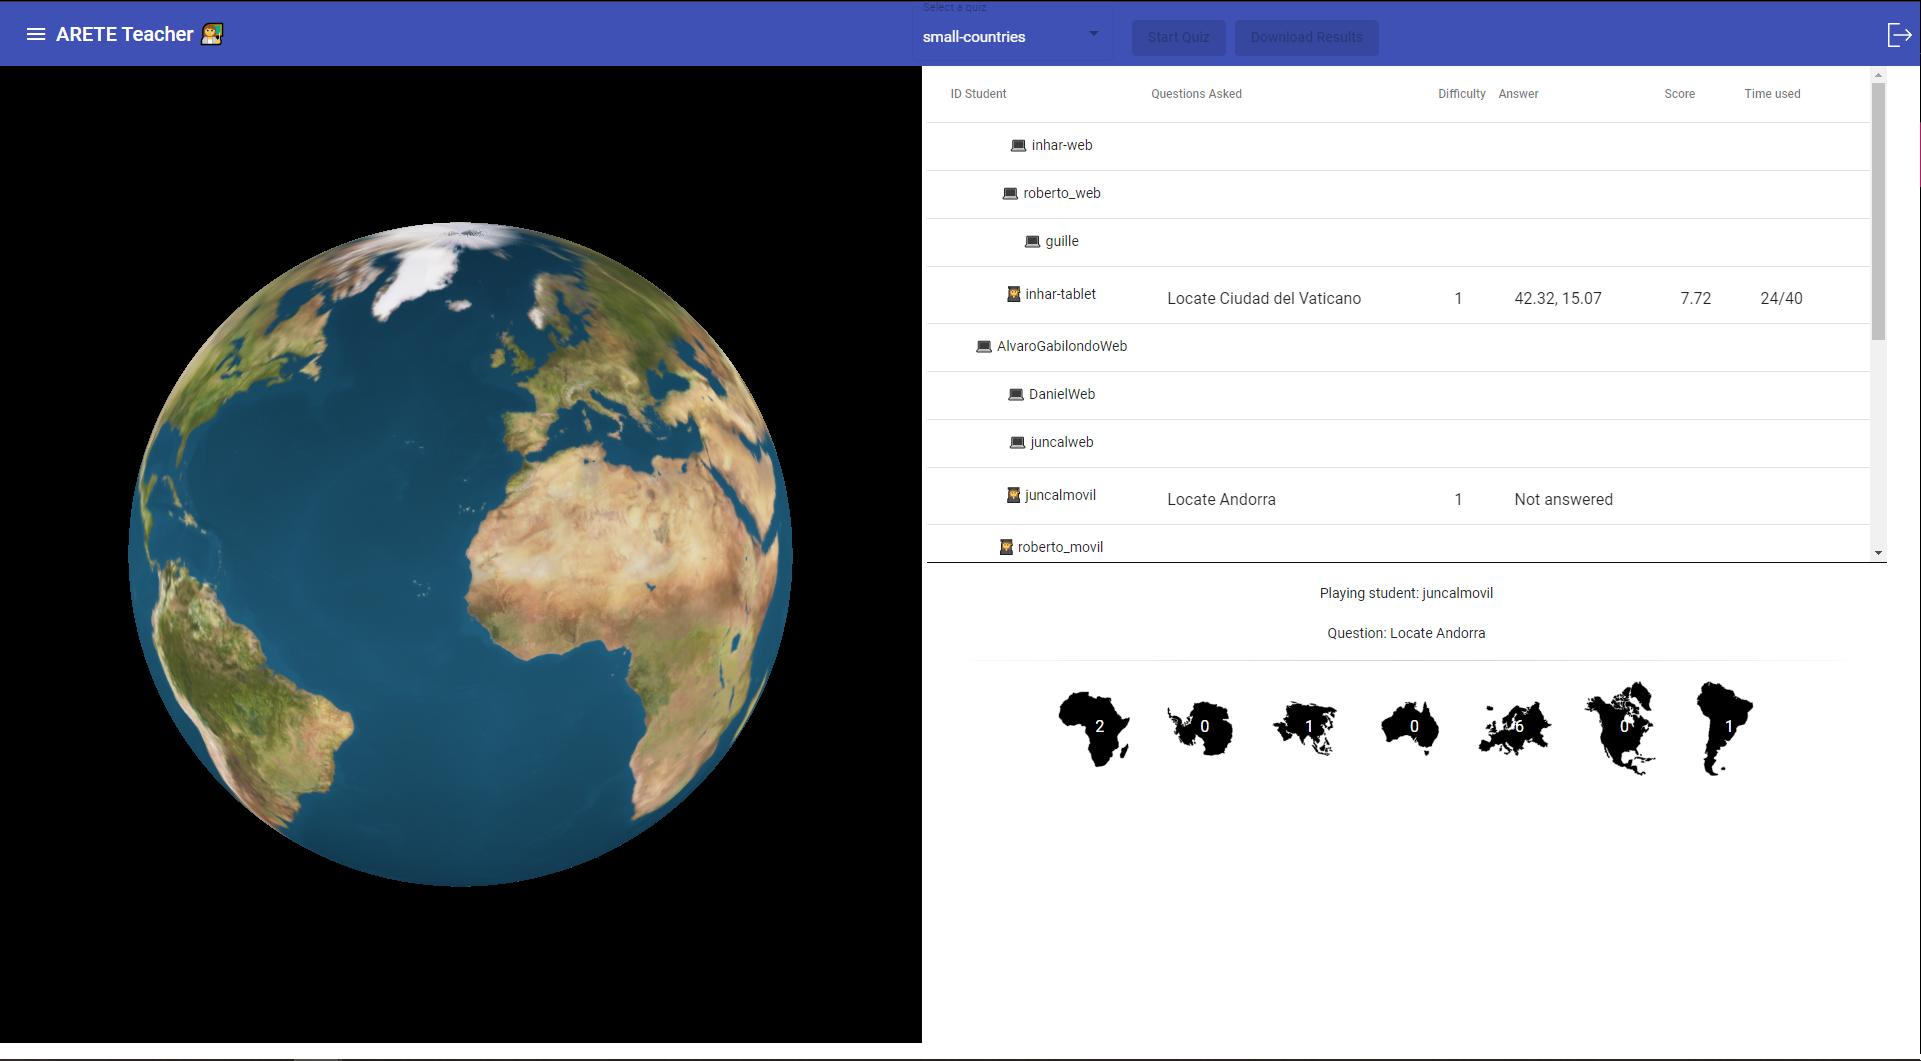
\includegraphics[width=0.95\textwidth]{Teacher_interface.png}
    \caption{\fontsize{10pt}{11pt}\selectfont{\itshape{The web-based teacher interface of the \appname{} application.}}}
    \label{fig:teacher_interface}
\end{figure*}

The application is designed to require minimal supervision from the teacher to let him or her interact as much as possible with the students.
As shown in Figure \ref{fig:teacher_interface}, the teacher interface consists of four parts:
\begin{itemize}
    \item A 3D representation of the augmented content as viewed by the active user (that is, the student who is answering the current question).
    \item The list of users connected to the app, together with the current score of the players and the last question they answered.
    \item The suggestions sent to the student currently answering the question.
    \item A dashboard (accessible in a separate tab) with charts of the scores achieved by each student across different sets of questions.
\end{itemize} 

The teachers who filled in the questionnaire described in Chapter \ref{chap:arch} mentioned that one of the factors limiting the usage of AR apps in schools is the lack of customisation capabilities.
In this respect, \appname{} provides an additional web interface from which the teacher can create new sets of questions.
To minimize the amount of work required by the teacher, the coordinates of each location are computed automatically using the Wikimedia API\footnote{\url{https://www.mediawiki.org/wiki/Wikimedia_REST_API}} and the questions are stored as JSON files, which are directly added to the application.
The interface of the \textit{watchers} is web-based, too, and has a look and feel similar to the teacher interface.

For the application to successfully achieve interoperability (\textbf{DO1}), several types of hardware as well as software libraries need to be supported.
In the aforementioned survey, the teachers reported a wide spectrum of devices available in their schools. Chromebooks and Android tablets were the most commonly used but other options included laptops, PCs, smartphones (both Android and iOS based) and iPads.
Furthermore, while none of the teachers reported using AR headsets such as HoloLens, it is believed that such devices provide the best AR learning experience for users. For this reason, the application supports Microsoft Mixed Reality Toolkit and is fully compatible with HoloLens devices.
The application for mobile and tablet devices has been developed using Unity 2020.3 and the AR functionalities are provided by the AR Foundation framework.
The web application has been built using Typescript and Three.js (to enable 3D content to be displayed in the browser). All the logging data and the statements collected during app usage are stored in a Mongo database in the Learning Locker instance deployed on AWS.
Porting to HoloLens and iOS devices is achieved through, respectively,  Unity integration with Microsoft MR Toolkit and by exporting the Unity project file to an XCode environment.

The application supports multi-user capabilities (\textbf{DO2}) by relying on the functionalities provided by the \arch{} architecture, which provides the \ork{} library for sharing 1-to-1 or broadcast message passing \citep{10.1007/978-3-030-93907-6_106} with minimal changes to the existing code base.
When a student is asked to answer a question, she becomes the active user. She shares the camera position (which determines her view of the 3D globe) as well as the position of the pin, once placed, with the other users.
The other students will then see, on their devices, the 3D globe in the same way the active user does.
For users on a mobile device this happens directly in the augmented space, while users using a PC will see the globe in a virtual 3D environment on a \texttt{\textless canvas\textgreater} element.
At the same time, suggestions from users are shared in a broadcast fashion, so that every student knows about the suggestions sent by others.
Finally, the teacher interface shares information about the current question, the score obtained by the active user after receiving her answer and the cumulative score of each user.
The information is shared 30 times per second and it allows a smooth \gls{ux} for every participant. The bandwidth usage is low since only basic data types such as strings and numbers are shared between users and the delay is below 15 milliseconds on both WiFi and mobile networks.
A previous approach tried to combine message passing and the transmission of the screen of the active user, using WebRTC, to the students using a PC to better simulate the AR experience \citep{UnityRenderStreaming}.
Unfortunately, such a solution has proven not to be scalable. Due to the poor support Unity has for WebRTC servers such as Janus, the application suffered delays which severely impacted the performance. With more than 5 users the UX was severely affected, and the app became unusable when more than 10 users were connected to the same session.

To comply with the data analytics design objectives (\textbf{DO3}, \textbf{DO4} and \textbf{DO5}) the application enables data collection through the storage of xAPI statements on a Learning Locker instance. 
Storing statements across each session enables the application to keep track of user activity and to store additional logging messages that simplify application debugging.
Learning Locker provides basic analytics and plotting capabilities through a web interface, as well as filtering and exporting the data in CSV format.
These functionalities have been extended through the development of a Python package\footnote{\url{https://stocastico.github.io/xapi_analysis/}} that includes methods to perform advanced data exploration and plotting, as well as running common machine learning models on xAPI statements data.
One of the aims of the package is to simplify data analysis as much as possible, enabling teachers without development skills to extract valuable information from the collected data.
For this reason, the package directly integrates GPT-4 \citep{openai2023gpt4, Osmulski_Ask_AI_-_2023}, so that users with a valid OpenAI Key can use natural language to debug or generate code when needed.
The package has been used to analyze the data collected during the evaluation of the app and the results will be presented in Section \ref{eval:results}.

Finally, to demonstrate how the aforementioned architecture enables developers to easily create multi-user applications (\textbf{DO6}), the developer of \appname{} was asked if and how the architecture helped him in the development process.
The developer mentioned that the architecture API enabled him to add multi-user functionalities in a transparent way. He neither had to deal with low-level networking issues nor implement platform specific methods.
While it was not possible to estimate the amount of lines of code or hours saved by using \arch{}, the developer said that he was satisfied with the capabilities of the architecture and would use it again for future projects.
Nevertheless, in order to enable teachers to create an ecosystem of collaborative AR applications for education, the developer mentioned that the availability of authoring tools to easily create applications on top of the \arch{} architectural design would be desirable.


%%%%%%%%%%%%%%%%%%%% EVALUATION %%%%%%%%%%%%%%%%%%%%%
\section{Evaluation}\label{eval:evaluation}

Our study aims to investigate how collaborative AR solutions may benefit the learning experience, and which are the usability issues of multi-user, multiplatform applications.
In the literature, unfortunately, there is no agreement on how to conduct evaluation of AR-based educational apps.
The survey from \cite{santos2013augmented} analyses 87 AR applications and the evaluation protocols included interviews, observing and coding overt behaviour and expert reviews.
Of those who used questionnaires, the majority crafted their own.
Among the works that used established questionnaires, some relied on the ISONORM Usability questionnaire \citep{prumper1999test}, Technology Acceptance Model \citep{davis1996critical}, Constructivist Multimedia Learning Environment Survey \citep{maor1999teacher}, Instructional Material Survey \citep{keller1987development}, Intrinsic Motivation Inventory \citep{ryan2000self}.
The number of participants in the evaluation of AR applications for education varies a lot depending on the study.
The systematic review of the literature published by \cite{masneri2020work}, of which Chapter \ref{chap:sota} represents an extension, shows that the number of participants varies between 2 and 290 participants. Another survey by \cite{santos2013augmented} analysed studies where the number of participants ranged from 4 to 419.

In this work, a questionnaire which adapts and extends the Positive System Usability Scale (P-SUS) \citep{brooke1996sus, sauro2011designing} was used. The questionnaire included a few additional questions to specifically evaluate the collaborative capabilities of the application.
The questions, presented in Appendix \ref{append:stuqu}, were grouped into 4 classes depending on what they were evaluating: the interest of the application as an educational tool, the usability of the app, its collaboration capabilities and its functionality.
Additionally, the participants could provide free-form feedback about the overall experience and whether they would recommend it to other students.
Finally, an interview with the teachers was conducted to collect their feedback about the learning experience, how collaboration may impact the involvement of the students, how  AR apps could be used to evaluate the students knowledge of a subject and how they would take advantage of the data collected through the application.

At the beginning of the evaluation, the participants were briefed about the experiment and its purpose and were asked to sign a consent form.
The questionnaires were anonymous but had an ID associated, so that during data analysis it was possible to associate the answers to the questionnaires with the data collected from each device through the xAPI statements.
The evaluation involved \numstudents/ students from \numschools/ educational institutions in San Sebastian (\textit{Colegio Salesianos Donostia}\footnote{\url{https://www.salesianosdonostia.com/es}}, \textit{IES Xabier Zubiri Manteo}\footnote{\url{https://zubirimanteo.hezkuntza.net/es/inicio}} and \textit{Universidad de Deusto}\footnote{\url{https://www.deusto.es/es/inicio}}) between March and May 2023.
Each experiment involved students of different ages (14, 17 and 19 years old) and their corresponding teachers.
None of the participants had previous experience with AR applications, but they were familiar with the hardware devices (smartphones, tablets and PCs) used during the evaluation.
In each school, the students were split into two groups: the first one represented the \textit{players}, tasked with answering the quiz questions using the application on mobile or tablet devices, while the second group represented the \textit{watchers}, who used a laptop or PC to see how the students answered the quiz and provided suggestions along the way.
Table \ref{tab:details_participants} shows the number of participants in each experiment, as well as details about the type of devices used when interacting with the application.

\begin{table*}[htbp]
\caption{\fontsize{10pt}{11pt}\selectfont{\itshape{Details of the demographics and number of devices used across each test.}}}
  \centering
  \begin{tabular}{l c c c c c c}
    \toprule
    \multirow{2}{*}{Participants} & \multicolumn{2}{c}{Gender} & \multicolumn{2}{c}{Players} & \multirow{2}{*}{Watchers} & \multirow{2}{*}{\textbf{Total}} \\
    \cmidrule(lr){2-3} \cmidrule(lr){4-5}
                            &  \multicolumn{1}{c}{Males} & \multicolumn{1}{c}{Females}  & \multicolumn{1}{c}{Tablets} & \multicolumn{1}{c}{Smartphones} & & \\
    \midrule
    14 year-old & 9 & 8 & 4 & 5 & 8 & \textbf{17} \\
    17 year-old & 16 & 1 & 3 & 6 & 8 & \textbf{17} \\
    19 year-old & 6 & 4 & 3 & 6 & 1 & \textbf{10} \\
    \midrule
    \textbf{Total} & \textbf{31} & \textbf{13} & \textbf{10} & \textbf{17} & \textbf{17} & \textbf{44}\\
    \bottomrule
  \end{tabular}
  \label{tab:details_participants}
\end{table*}

Once each participant had a device assigned, they were asked to connect to the application by selecting the session ID representing the experiment and the user ID. The latter would be used as the \textit{Actor} value for the xAPI statements generated while using the application.
After a short Q\&A session to clarify doubts about the app usage the teacher started the quiz and the students would then take turns to answer two sets of questions.
Once the quiz was over, the teacher stopped the data collection and was able to check the score of each student and to export the data.
After logging out of the session, the students filled in the questionnaires while the post-study interview with the teacher was conducted.


%%%%%%%%%%%%%%%%%%%% RESULTS %%%%%%%%%%%%%%%%%%%%%%%%
\section{Results and Discussion}\label{eval:results}

In this Section, the results of the survey as well as the data collected from the app are presented and discussed. An extended version which also includes a subgroup analysis of the data split for different age group, is available in the code and data repository\footnote{\url{https://github.com/Stocastico/Evaluation_paper}}. The quantitative results from the responses to the post-intervention survey (shown in Appendix \ref{append:stuqu}) are summarised in Figure \ref{fig:survey_all}. They are shown as stacked bar charts \citep{friedman1999rating}, where the chart on the left  refers to the answers to each question and the chart on the right to the groups of questions mentioned in Section \ref{eval:evaluation}.
From the figure it can be appreciated that the application was very well received by the students and that every question except the first one was answered positively (\textit{Agree} or \textit{Strongly agree}) more than 60\% of the time.
The average rating for each question ranges from $3.45$ to $4.43$, with limited variability across answers, with the standard deviation being below 1 for most of the questions.
The plot on the right in Figure \ref{fig:survey_all} shows similar results: the students assigned the highest score to questions related to Usability, especially question 2 (\textit{I found the application to be simple}) and 3 (\textit{I thought the application was easy to use}). The questions related to Functionality received a high score as well, while the ones relating to the Educational content of the app show the highest variability: those questions received the highest amount of negative answers while also receiving the highest score more than 40\% of the time. 

\begin{figure*}[htbp]
    \centering
    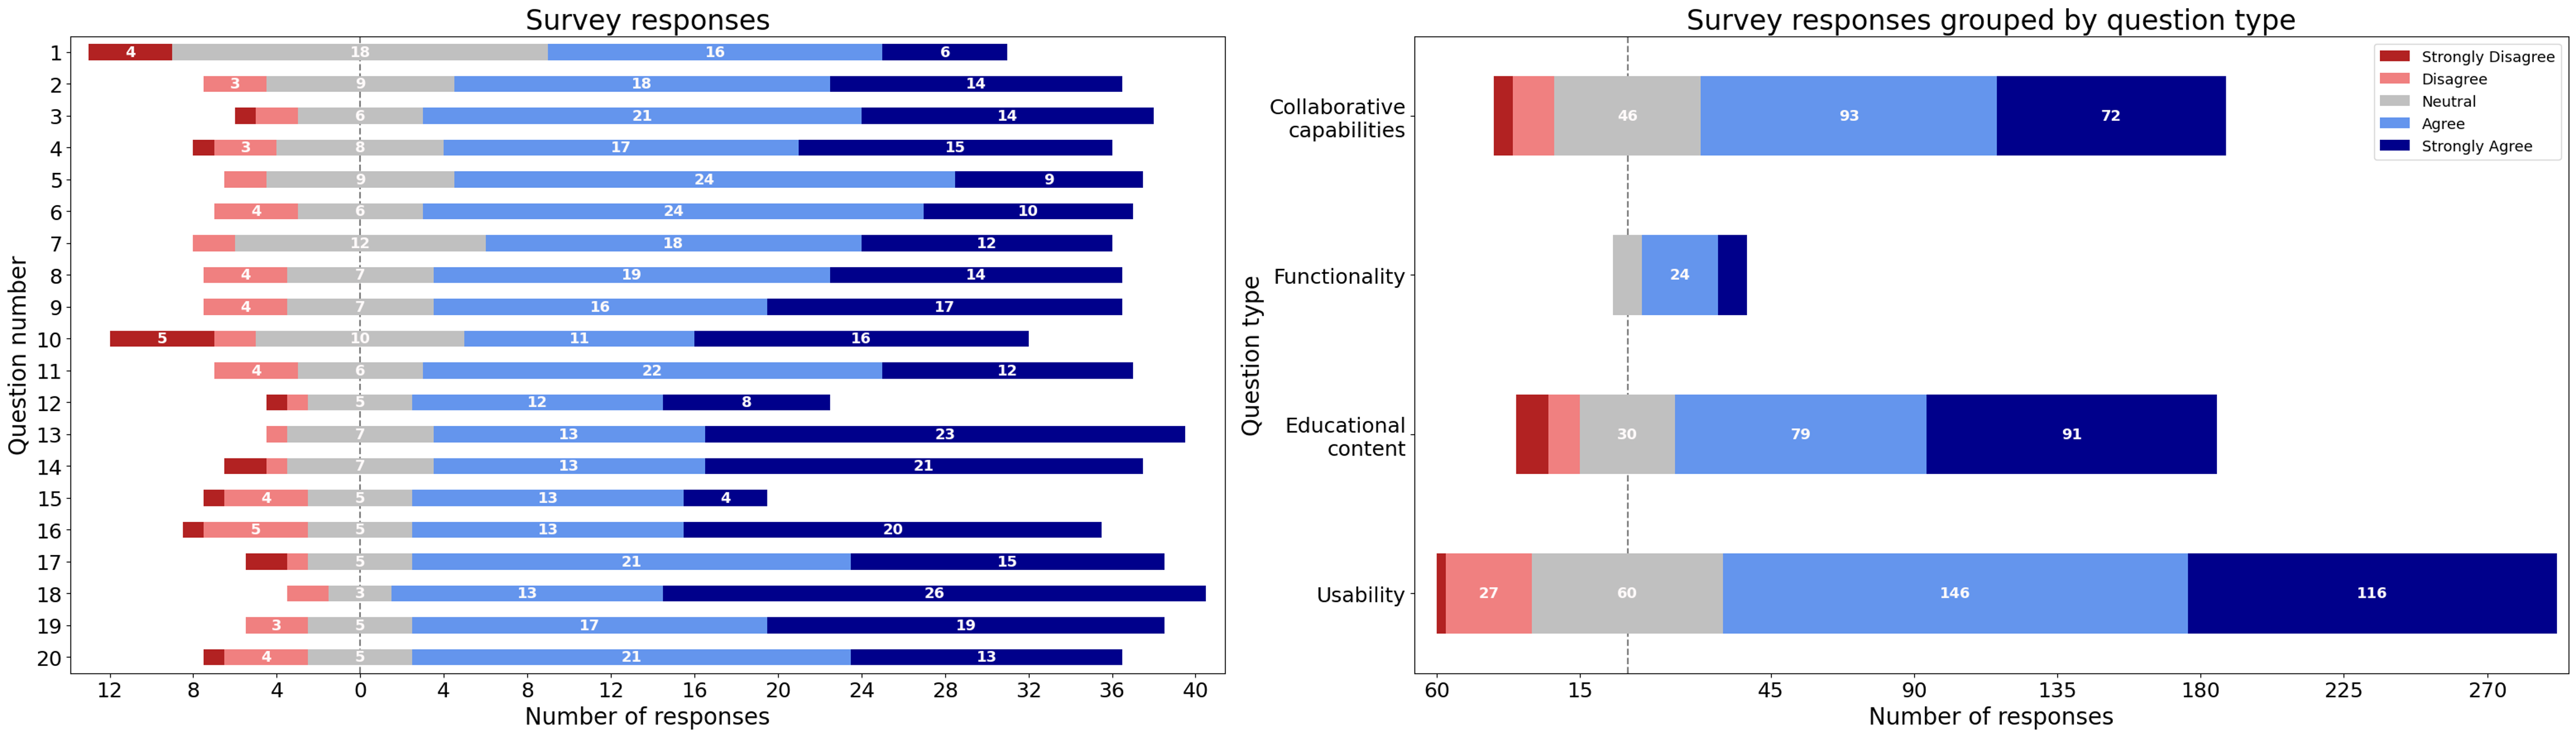
\includegraphics[width=0.95\textwidth]{survey_results_2.png}
    \caption{\fontsize{10pt}{11pt}\selectfont{\itshape{Left: survey results on each question. Right: survey results grouped by question type.}}}
    \label{fig:survey_all}
\end{figure*}

The bar plots of Figure \ref{fig:survey_split} are used to identify differences in the answers of the students, based on their role when using the app and the device they used.
Somewhat surprisingly the \textit{watchers} gave a slightly higher mean score, albeit with a much higher variability in the answer.
As for the device type, the users on an Apple device (iPhone or iPad) gave a higher score compared to students using an Android device or a PC, but the differences are not statistically relevant.

\begin{figure*}[htbp]
    \centering
    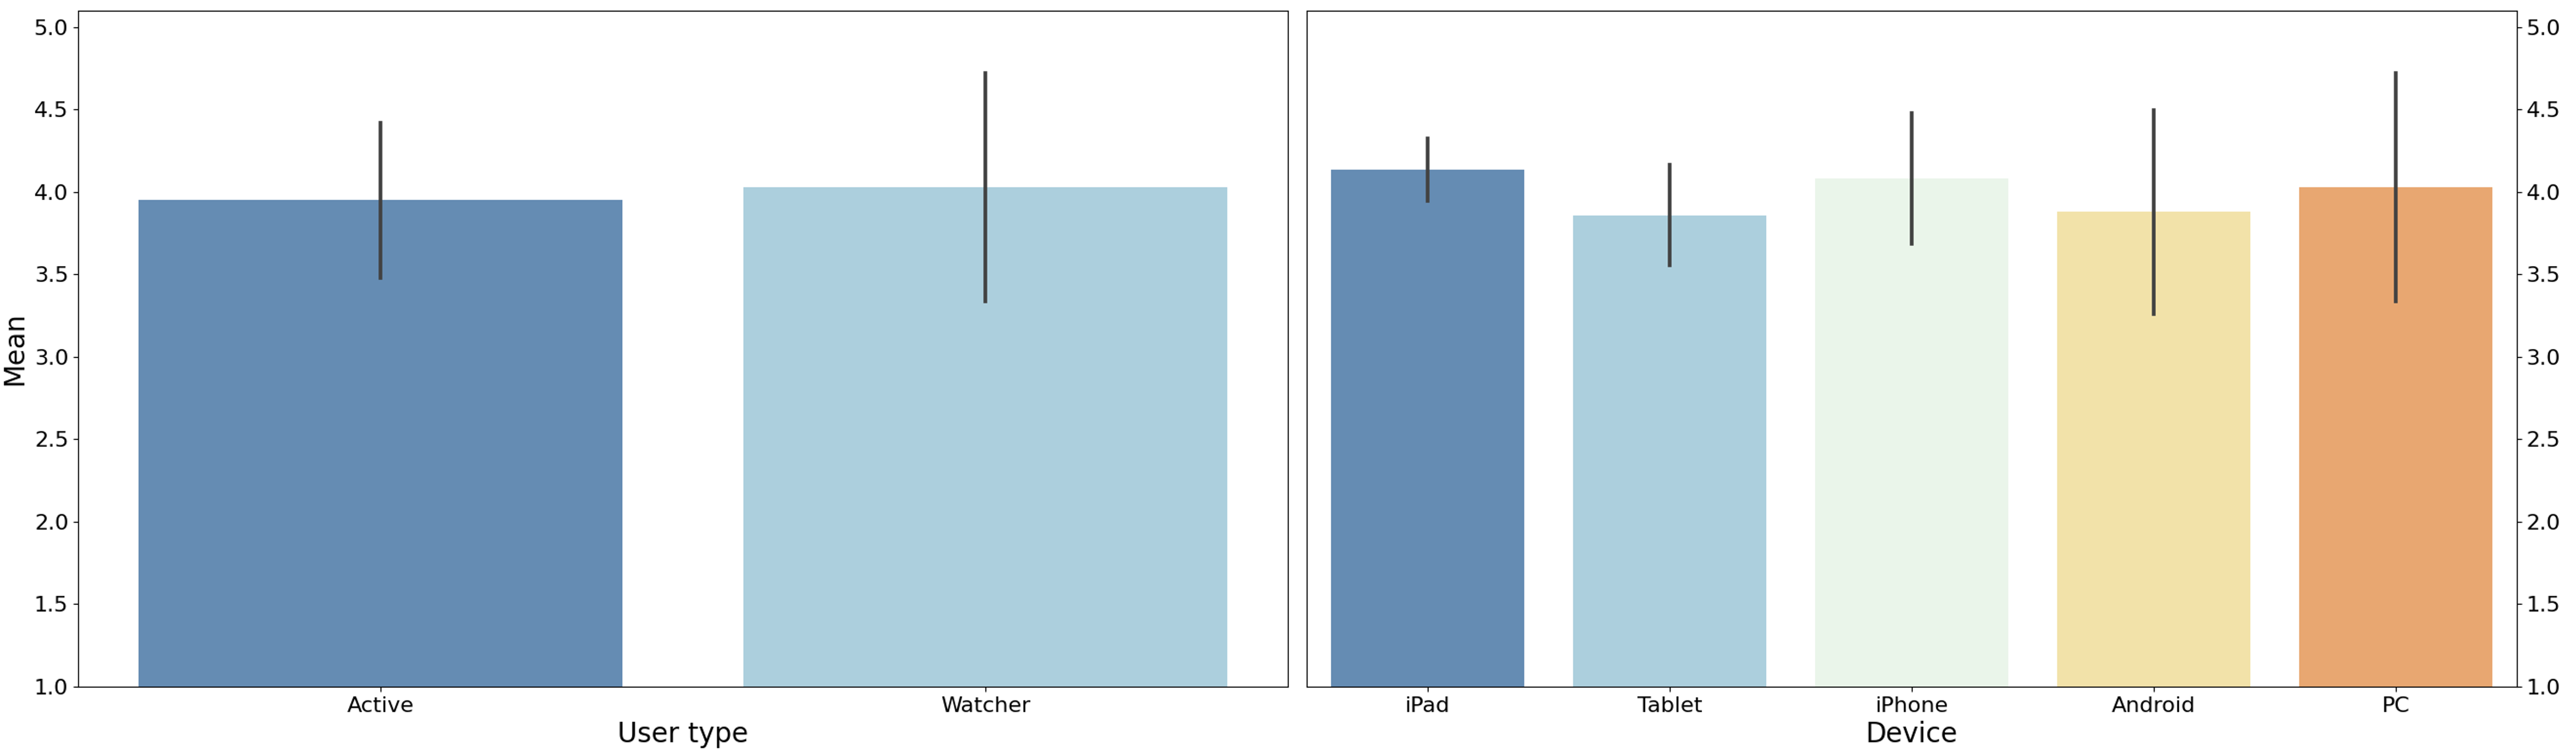
\includegraphics[width=0.95\textwidth]{survey_results_type_2.png}
    \caption{\fontsize{10pt}{11pt}\selectfont{\itshape{Mean score of the questionnaire answers. The vertical bars represent the standard deviation.}}}
    \label{fig:survey_split}
\end{figure*}

Figure \ref{fig:survey_split_grouped} shows the mean score and the standard deviation for the questionnaire answers grouped by user.
It shows the split of the students by age, their role when using the app and the device they used.
From this visualization an outlier can be easily identified, represented by the only student in the 19 year-old group who used a PC and was the only non-active user in that session.
The reason for the lower score, as identified by the comments provided by the student in the questionnaire, was that the experience for him did not feel particularly immersive nor collaborative, as his role was fairly different from that of his classmates. 

\begin{figure*}[htbp]
    \centering
    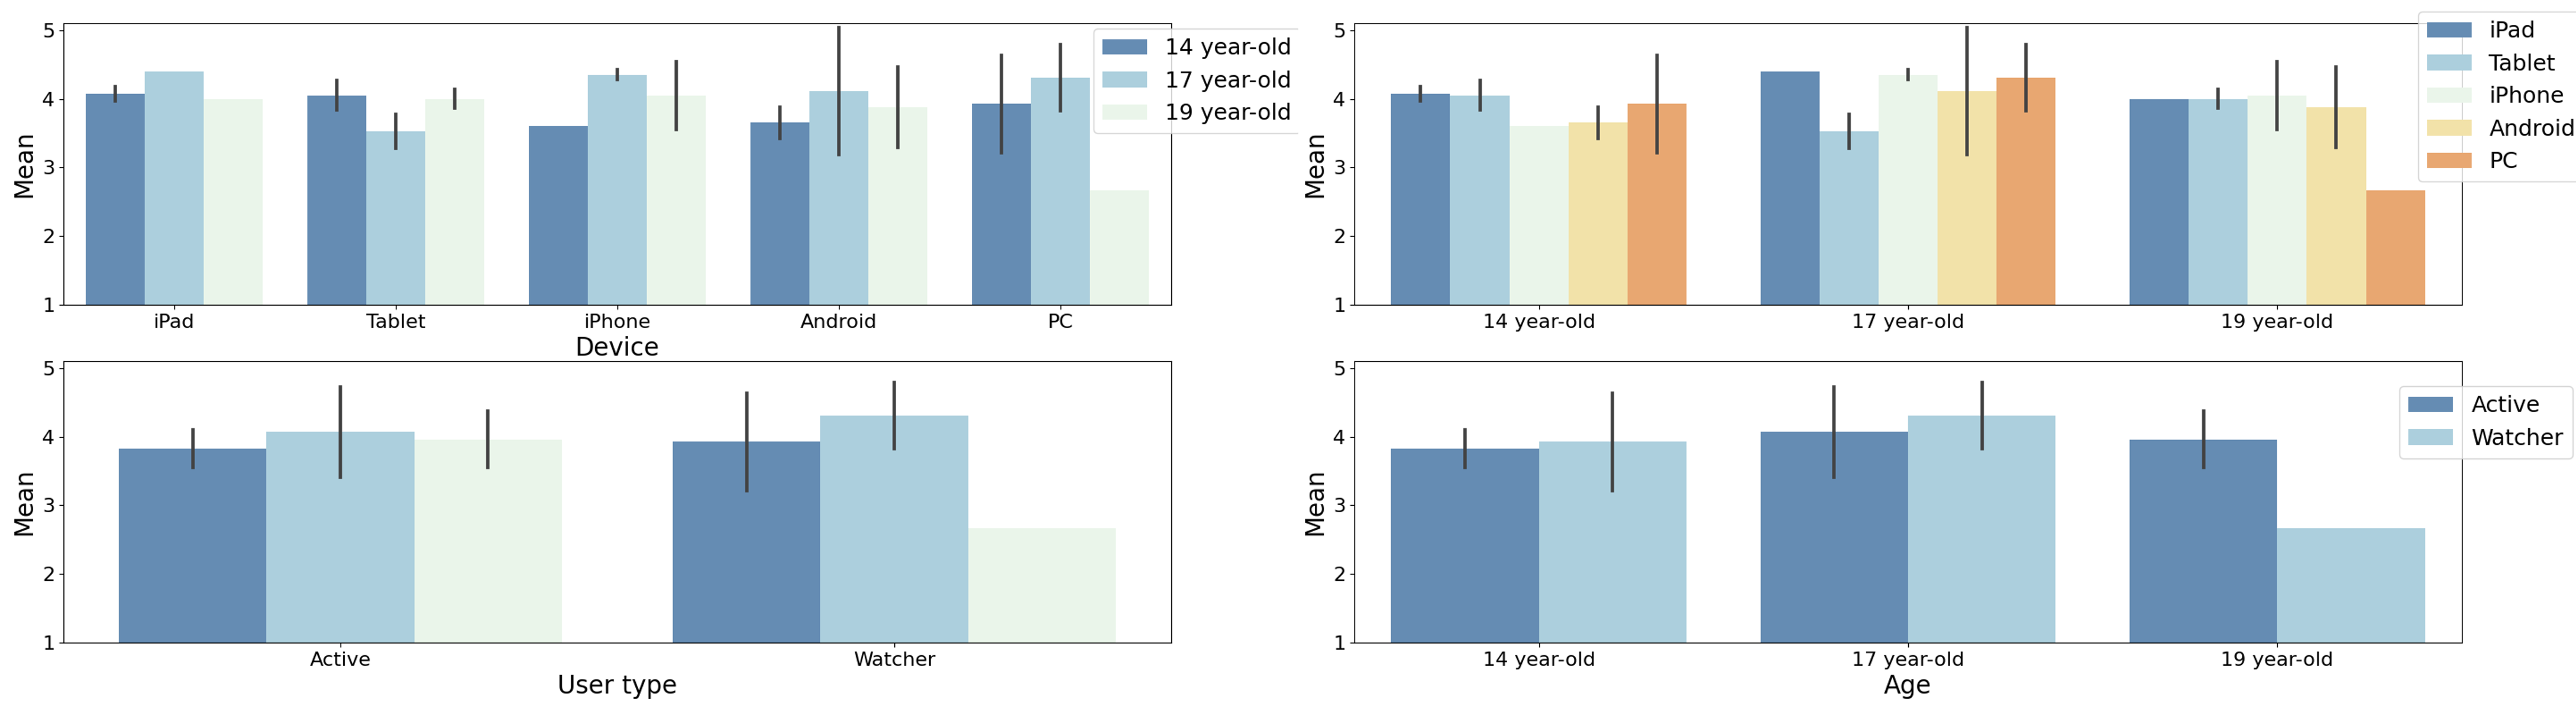
\includegraphics[width=0.95\textwidth]{survey_results_grouped_2.png}
    \caption{\fontsize{10pt}{11pt}\selectfont{\itshape{Survey results split by user type. Left: Average question score by device used and student role. Right: Average question score by students age.}}}
    \label{fig:survey_split_grouped}
\end{figure*}

Since \appname{} collected data in the form of xAPI statements, an analysis of the data received was conducted. This showed that there is a correlation between the score in the questionnaire and the number of statements collected by the application for each user.
The actions registered by the app include both interactions between students, such as the suggestions sent, and the interactions of a user with the app.
As shown in Figure \ref{fig:num_interactions}, there is a high variability in how much the students interacted. It is clear, though, that the \textit{players} (the students using a mobile device and interacting with the augmented content) were much more involved in using \appname{}. This is probably because their role was much more interactive and immersive.

\begin{figure}[htbp]
    \centering
    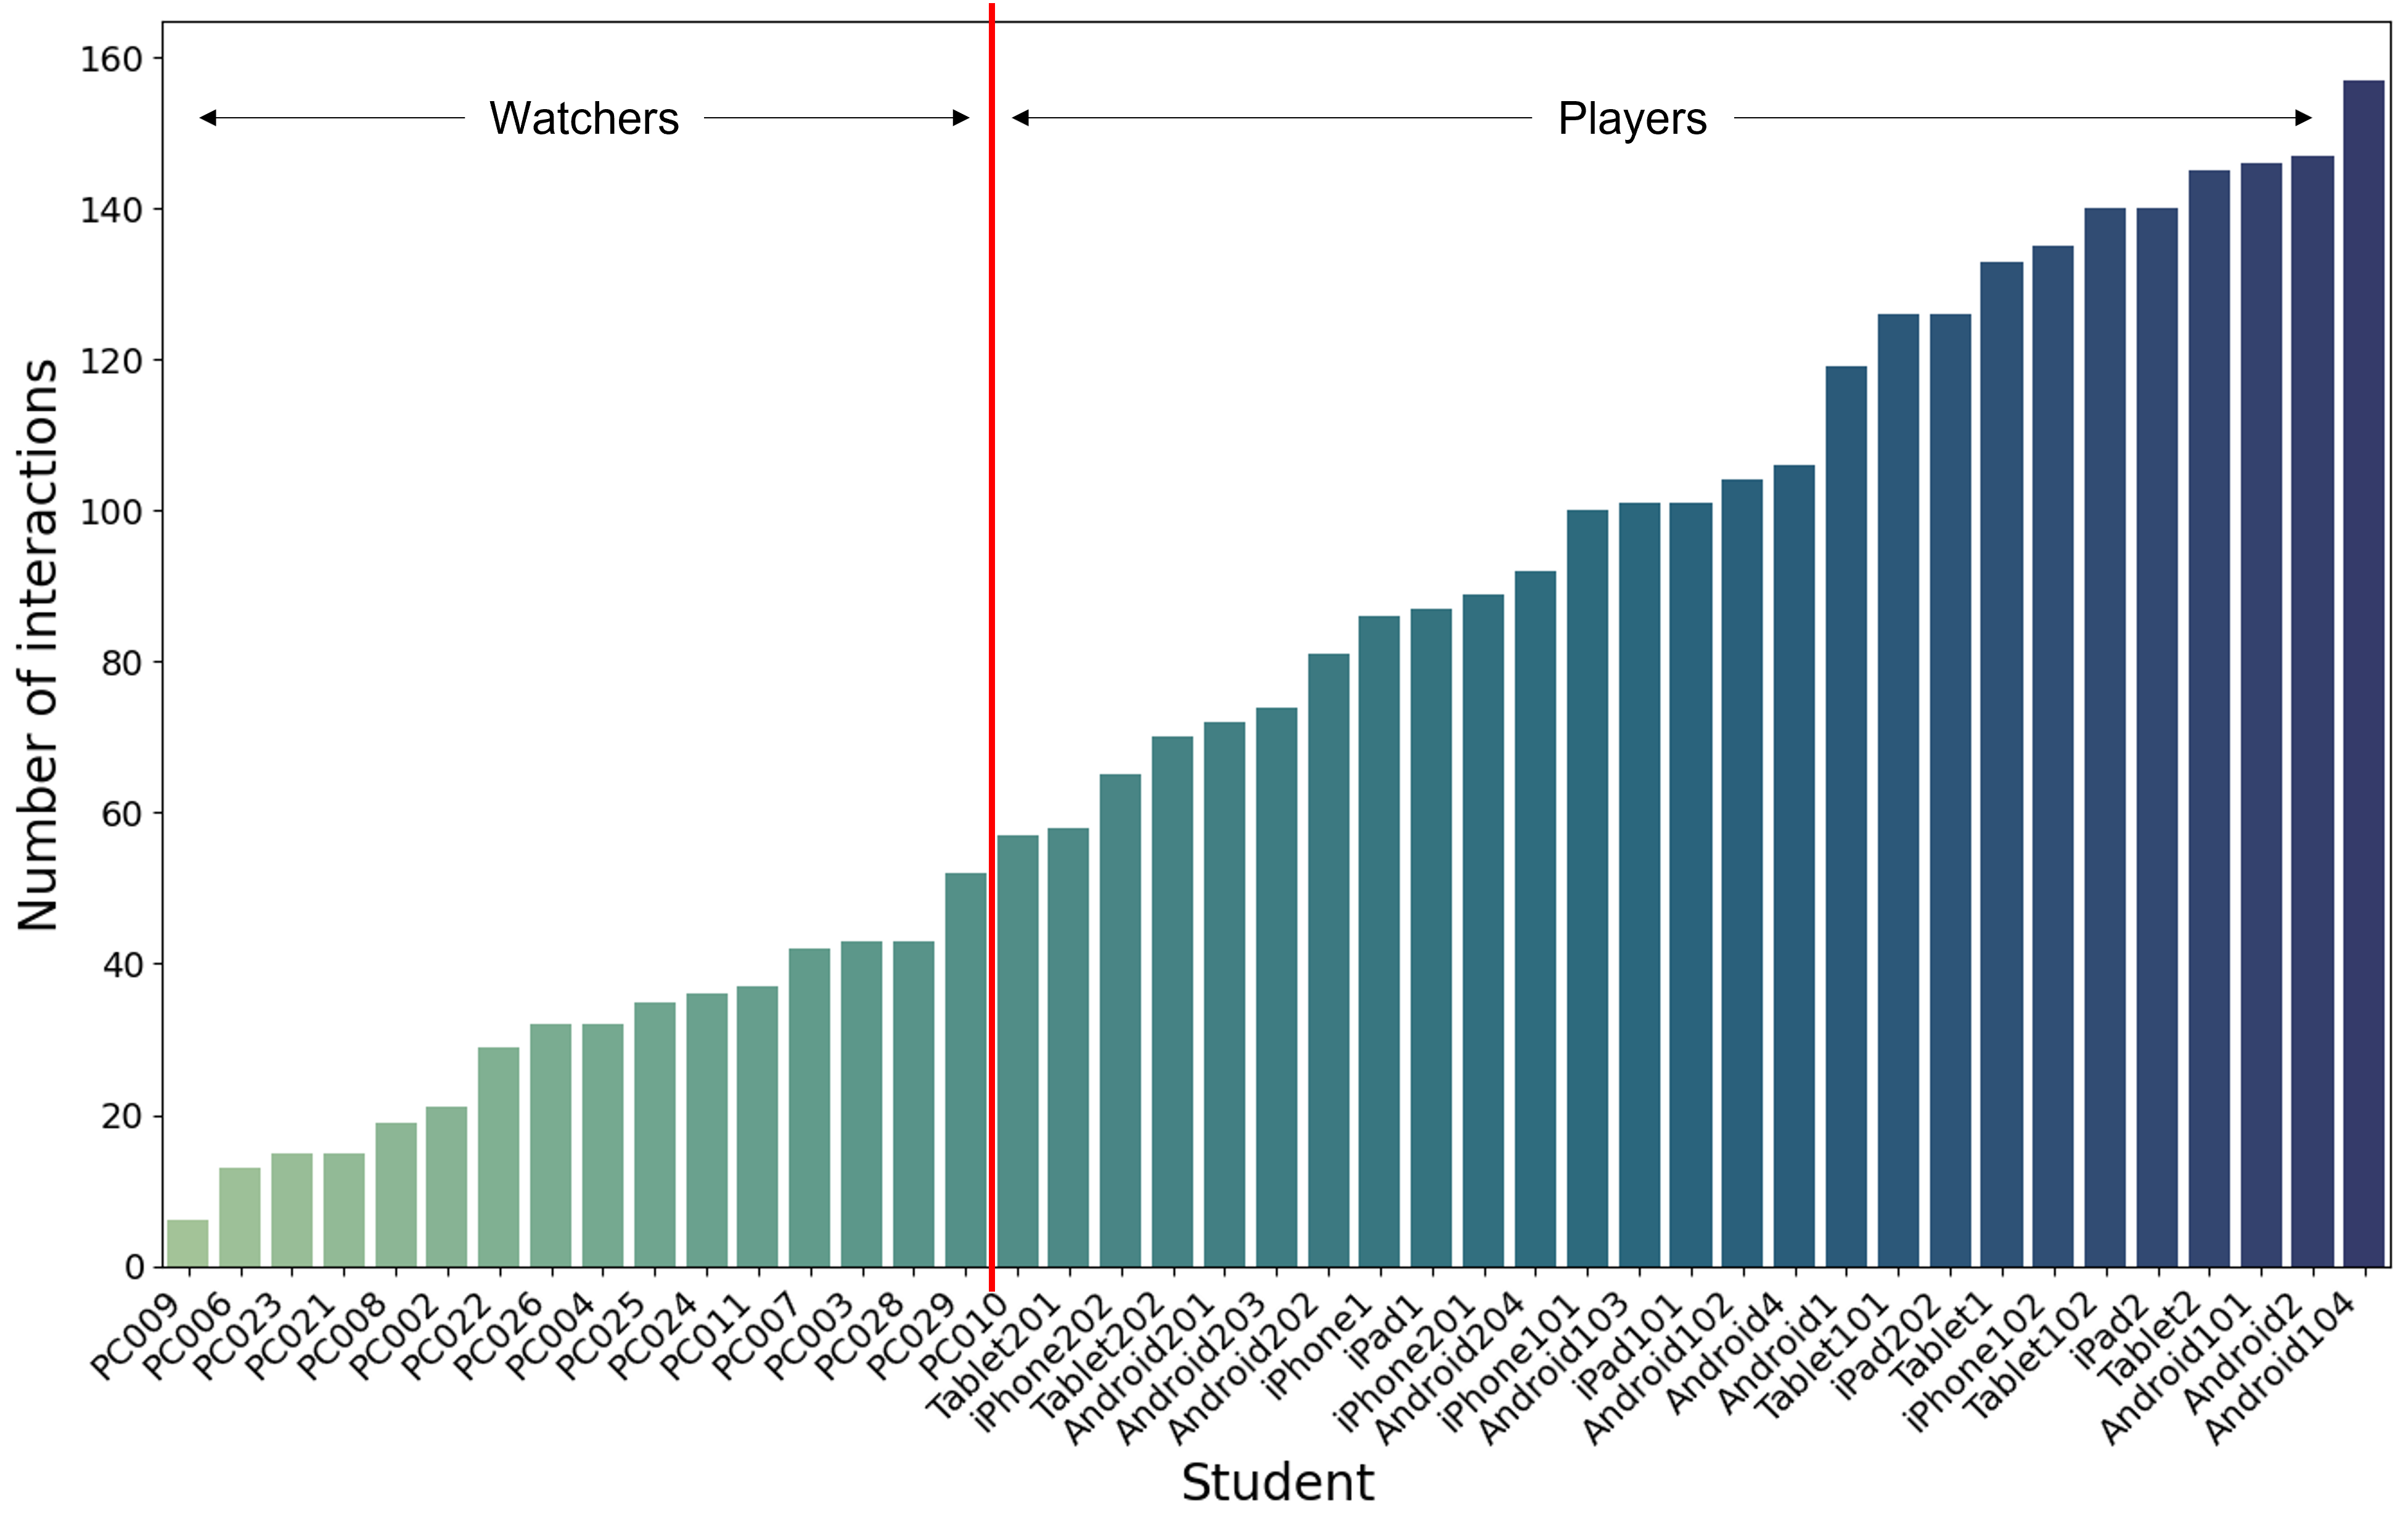
\includegraphics[width=0.95\textwidth]{num_interactions_2.png}
    \caption{\fontsize{10pt}{11pt}\selectfont{\itshape{Interactions with the application for each student (identified by the device used).}}}
    \label{fig:num_interactions}
\end{figure}

An interesting aspect to analyse is whether there is any correlation between the number of interactions of each student and the answers they have given to the survey questions.
Two statistical approaches were followed.
First,  a correlation analysis was performed to check whether there was a relation between the number of interactions and the average scores given to the questions by the students, by calculating the Pearson correlation coefficient.
The second approach is that of hypothesis testing. This checks whether the answers given by students with a high number of interactions are significantly different from the answers given by students who had a low number of interactions.
A two-sample T-test assuming equal variances has been used for testing \citep{welch1947generalization}.
In both cases, a significance level of $p < 0.05$ was established.
Since the interactions between the \textit{watchers} (students on a PC) and \textit{players} (students on a mobile device) are significantly different, it was also performed an analysis for these specific subsets of the data as well.

Unfortunately, the analysis performed is not conclusive.
None of the tests returned a p-value below the significance level, and the correlations identified (most notably between the interactions of students on a PC and their answers to the survey) are not statistically significant.

A similar analysis was conducted to inspect whether there were correlations between the score obtained in the quiz and the answers in the survey. In this case as well, no statistically significant correlation was found.
This was  expected since the app was designed to ask questions of varying difficulties, but the difficulty level of the questions received by a student did not change during the test.
As expected, students who received easier questions achieved a higher score and there is indeed a significant correlation between these two variables.

Another interesting correlation to analyse was the one between the mean score obtained in the survey and the number of suggestions sent by the user.
The statements about suggestions are an interesting variable because for each question, every user (besides the \textit{active player}, the one answering the current question) was able to send two suggestions.
For this reason, many such statements were collected during the trial.
To encourage students to provide suggestions, the application assigned points for each correct suggestion.
In this case the analysis showed a significant positive correlation ($r = .37$, $p = .044$), meaning that the most engaged students were the ones that gave a higher score in the survey.

Finally, a clustering analysis of the data was performed, to check if it is possible to identify distinct groups of users.
In this case, the focus was only on the students who used a mobile device, since they provided a greater number of features to work with.
The average time left per question, the number of suggestion accepted, the total number of interactions and the mean value of the answers in the survey were the four variables considered.
A dimensionality reduction using PCA \citep{jolliffe2002principal}, shown on the left in Figure \ref{fig:clustering}, revealed that the first two principal components explained more than 70\% of the variance in the data.
Additionally, a biplot analysis indicated that the most relevant variable for the first principal component was the number of user interactions, while for the second one it was the results of the survey.

As the number of data points is small, a hierarchical clustering algorithm \citep{hiera} was used.
A Silhouette score \citep{ROUSSEEUW198753} computed for cuts between 2 and 6 suggested that the optimal number of clusters in this case was either 2 or 4.
The clustering results (shown in Figure \ref{fig:clustering}, right) identified one big group of students characterised by having a particularly high number of interactions and another one having a higher score in the survey answer.
The other two clusters were harder to characterise.
In one case it was not possible to clearly identify a common feature in the data, while in the other the cluster only contained two members, and the intra-cluster variable suggests that those data points are probably outliers.

After running the trials in the educational institutions, a post-intervention interview with the teachers was conducted.
The 3 teachers seemed very intrigued by the possibility of easily being able to use AR in school without having to resort to any specific hardware. They especially valued the fact that the collaborative features of \appname{} encouraged the students to work together to provide the answer, either through the features of the application or simply by talking to each other.
Another relevant point for the teachers was the possibility of adding new content on their own, as well as the fact that they could export the results to the school \gls{lms}.
The teachers were more sceptical about the AI features provided by the backend. They mentioned that the vast majority of their colleagues do not have sufficient knowledge to perform the analysis on their own. They would rather prefer using a PowerBI or Tableau interface to visualise data and extract basic reports.
The teachers also mentioned that the role of the \textit{watchers} was too passive and that in longer experiments these students might lose interest. They suggested enabling the role of active user when using a PC, even if that means not using AR components but a browser-based 3D graphics library.

\begin{figure*}[htbp]
    \centering
    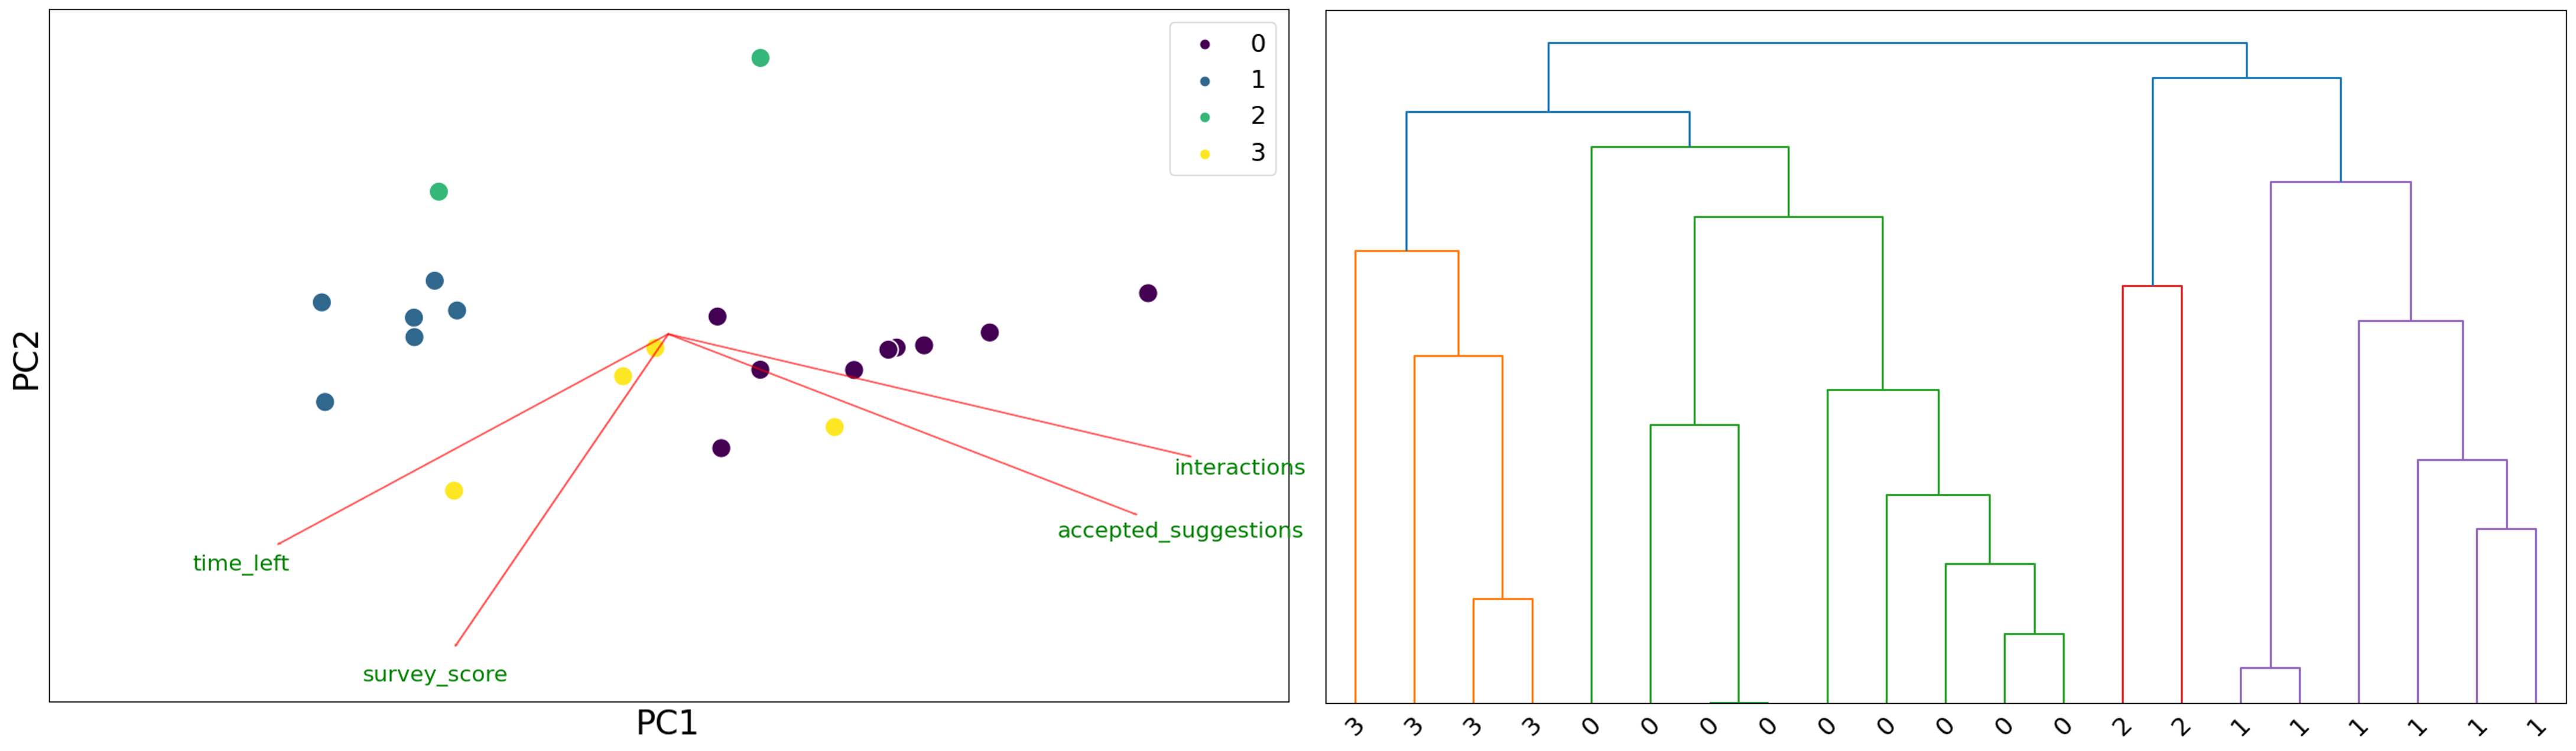
\includegraphics[width=0.95\textwidth]{unsup_3.png}
    \caption{\fontsize{10pt}{11pt}\selectfont{\itshape{Left: Clustering of the active users data on the PCA space. Right: the dendrogram representing the hierarchical clustering.}}}
    \label{fig:clustering}
\end{figure*}

%%%%%%%%%%%%%%%%%%%% CONCLUSIONS %%%%%%%%%%%%%%%%%%%%
\section{Final remarks}\label{eval:conclusion}

In this Chapter, \appname{} was presented, a multiplatform AR application which implements collaborative capabilities and gamification concepts. The application is based on a Geography quiz and it fulfils the design objectives identified in Chapter \ref{chap:arch}.
The evaluation, conducted with 44 students and 3 teachers, and the analysis of the xAPI statements showed that students evaluated very positively the application.
Additionally, it was measured a small but statistically significant correlation between the ratings in the questionnaire and the engagement of the students. Furthermore, post-study interviews with the teachers identified the collaborative capabilities and the possibility of personalising the app content as being key factors for a sustained usage of AR apps.
In fact, one of the teachers suggested the possibility of adding more collaborative features, such as a chat system or speech-based interactions to make the application more immersive and more appealing when used in a distributed setting.



